\documentclass[12pt,a4paper]{article}
%%%%%%%%%%%%%%%%%%%%导言区%%%%%%%%%%%%%%%
%%宏包设置
\usepackage[BoldFont,SlantFont]{xeCJK}
\usepackage[dvips]{graphicx}
%\usepackage{hyperref}
%%字体设置
\setCJKmainfont[BoldFont=SimSun,ItalicFont=SimSun]{SimSun}
\setmainfont{Times New Roman}
\setCJKfamilyfont{ht}{SimHei}
%%页面设置
\addtolength{\hoffset}{-1cm}
\addtolength{\voffset}{-2cm}
\addtolength{\textheight}{4cm}
\addtolength{\textwidth}{2cm}
%%标题页
\title{NIOS II Linux Tutorial}
\author{作者:陈锋 \ {}\ {} 邢岚}
%%%%%%%%%%%%%%%%%%%%正文%%%%%%%%%%%%%%%
\begin{document}
\thispagestyle{empty}
\maketitle{}
%%%%%%%%%%%%%%%%%%%%前言%%%%%%%%%%%%%%%
\section{前言}
本文由\textbf{texlive 2010}构建.

这是一个\textbf{NIOS II Linux}开发的入门教程,拟包括以下几个部分:\footnote{随着编写计划的变化,可能会有增减.}
\begin{itemize}
\item 介绍\textbf{NIOS II Linux}开发环境;
\item 一个完整的流程;
\item 创建自己的SOPC系统和Linux内核;
\item linux下驱动开发举例;
\item linux下普通应用程序开发;
\item FTK应用程序开发;
\end{itemize}
%%%%%%%%%%%%%%%%%%%%构建开发环境%%%%%%%%%%%%%%%
\newpage{}
\section{构建开发环境}
2009年9月,nioswiki社区推出基于NIOS II处理器的linux内核开发包,为开发者提供一种新的系统方案.

使用\textbf{NIOS II Linux}开发需要搭建硬件和软件环境.目前已知的开发环境有两类:
\begin{table}[!hbtp]
\centering
\begin{tabular}{|l|p{0.68\textwidth}|}
\hline
完全在linux下开发 & 在linux下安装linux版本的Quartus II和NiosII IDE开发工具,同时安装nios-linux内核开发包.
据我所知目前只有\textbf{Ubuntu9.04}可以兼容,Ubuntu9.10及以上版本暂时不支持\footnote{不支持的原因是nios2-download脚本在Ubuntu9.10及
以上版本中部分无法执行.而官方推荐的Redhat企业版和Fedora等均可配置.};\\
\hline
WindowsXP+Linux虚拟机 & 这种方案更适合大多数平时工作在Windows环境下的开发者.本文接下来将介绍这种方案的配置;\footnote{由于在linux下
的usb-blaster驱动比windows下性能要相对差些,当构建的系统选择以JTAG-UART作为终端时,在linux环境下的``nios2-terminal''命令会导致系统阻塞,此时
我更倾向于使用本方案.} \\
\hline
\end{tabular}
\end{table}
%%%2.1
\subsection{硬件环境}
首先需要在Windows上安装Quartus II和相应版本的NiosII IDE.本文使用是9.0版本.因此大于等于该版本都应该没有问题.
安装过程这里不赘述,有问题请自行查阅相关文档.但是安装的版本{\CJKfamily{ht}需要有lisence支持}.
%%%2.2
\subsection{软件环境}
linux内核驱动和应用程序的开发需要在类Unix操作系统下进行,最普遍的就是Linux操作系统.这里我们选择流行程度最高的Ubuntu操作系统作为开发平台.

首先我们要安装一款虚拟机软件\footnote{Windows下有Vmware,Virtual Box等}.通过该软件创建虚拟机并安装Ubuntu.安装好的虚拟机系统要满足两个要求:
\begin{itemize}
\item 能够连接互联网,下载内核开发所需的文件;
\item 能够与宿主机(Windows)交换文件.宿主机下生成的头文件要传入虚拟机中交给内核开发包使用,而虚拟机下生成的内核可执行文件要
在window下通过nios shell下载;
\end{itemize}

我们以Virtual Box为例说明如何操作\footnote{使用Vmware等只要满足上面两个条件同样可以搭建开发环境}.
%%%2.2.1
\subsubsection{虚拟机安装Ubuntu并做相关设置}
创建虚拟机之前,本地电脑上需要准备如下内容:
\begin{itemize}
\item Ubuntu安装光盘或ISO镜像文件;
\item 已安装好Virtual Box软件;
\item 足够的硬盘空间(14G左右);
\end{itemize}

在Virtual Box主页面菜单上选择\fbox{控制-->新建},操作系统类型选择\textbf{Linux},版本选择\textbf{Ubuntu},如图\ref{f_create_vb1}所示.
\begin{figure}[!bthp]
\centering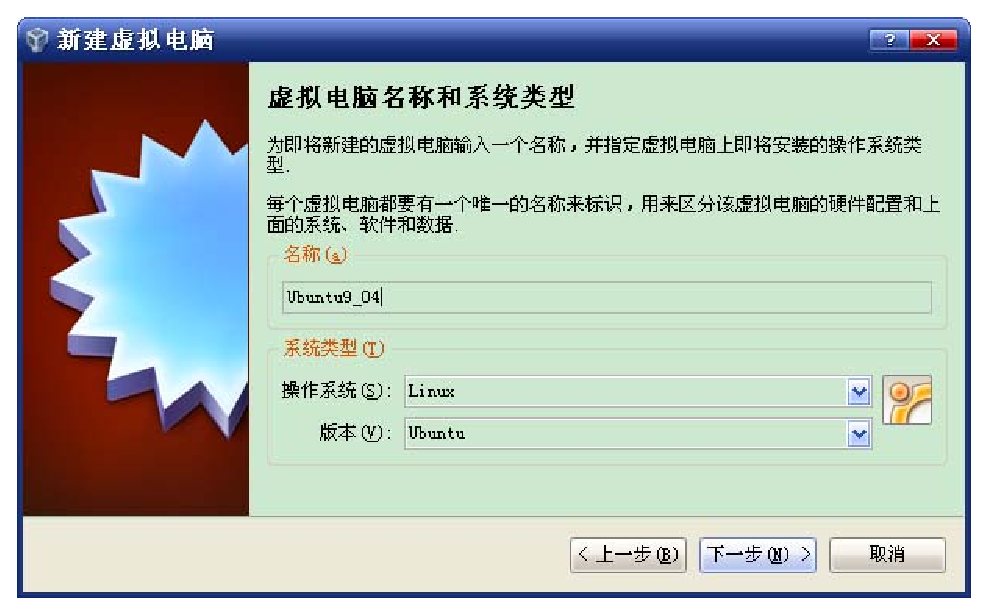
\includegraphics[width=1\textwidth]{pic/f_create_vb1.eps}
\caption{创建虚拟机:整体设定\label{f_create_vb1}}
\end{figure}
内存选择为当前系统内存一半略少,尽量发挥系统性能.硬盘选择"创建新的虚拟硬盘"并选择"固定大小"\footnote{相对于动态增长,
固定大小使得虚拟机运行速度更快}.硬盘大小至少10G,以免内核开发包在虚拟机中解压缩后空间不够,{\CJKfamily{ht}注意,默认虚拟硬盘保存在系统盘中,
请将位置改到有足够空间的磁盘上}.硬盘创建完成后确定即可.

到现在为止,虚拟机已经创建完毕.但是当前的虚拟机内没有任何系统,甚至连分区都没有,此时需要通过光驱安装操作系统.本文使用ISO镜像
文件进行安装.

在没有运行虚拟机的情况下,点击\fbox{设置}图标,右侧找到"介质"一栏,对ISO进行注册.如图\ref{iso0},\ref{iso1}和\ref{iso2}所示.
\begin{figure}[!bthp]
\centering
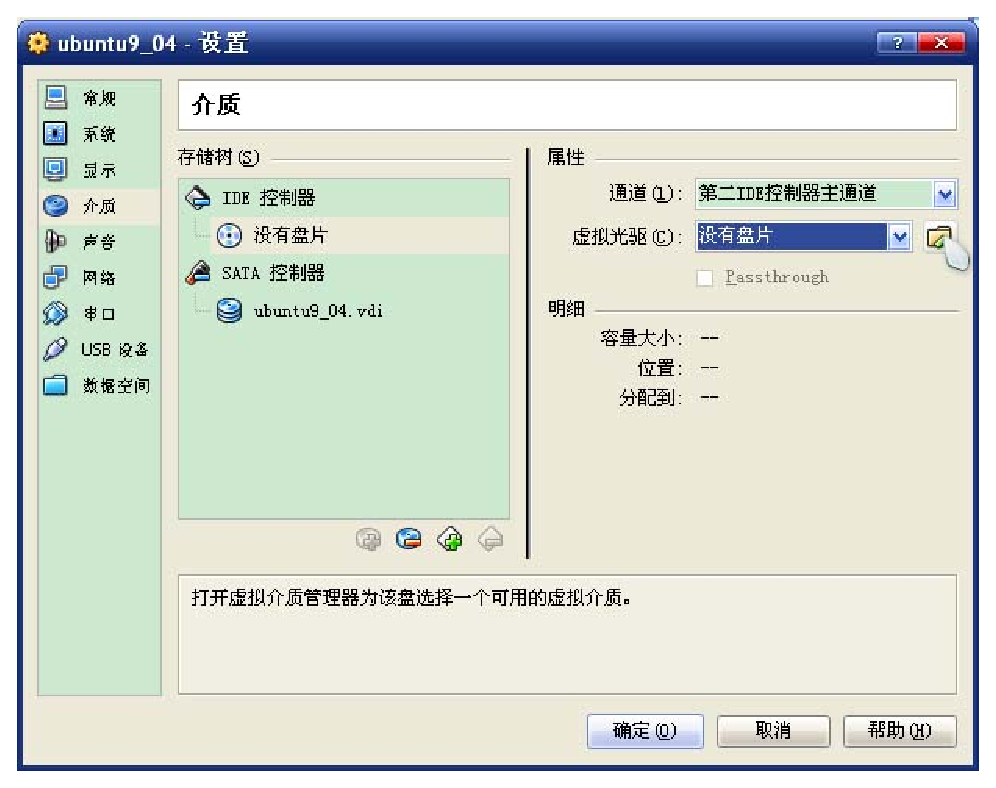
\includegraphics[width=0.8\textwidth,scale=0.8]{pic/f_vb_setting_iso.eps}
\caption{设置ISO\label{iso0}}
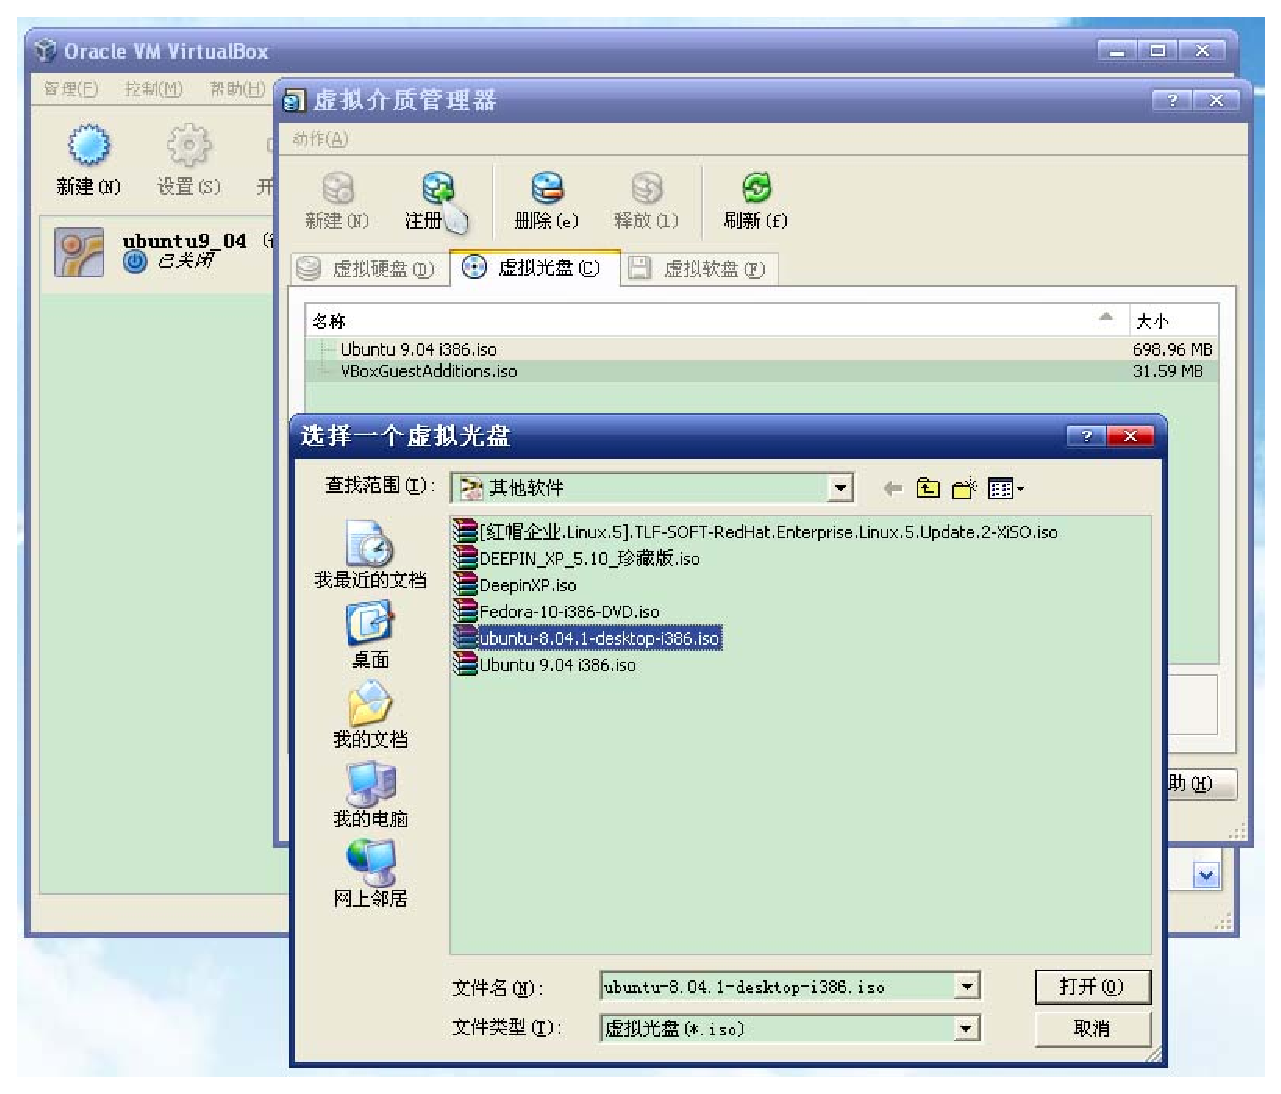
\includegraphics[width=0.8\textwidth,scale=0.8]{pic/f_vb_setting_iso_register.eps}
\caption{设置ISO\label{iso1}}
\end{figure}
\begin{figure}[!bthp]
\centering
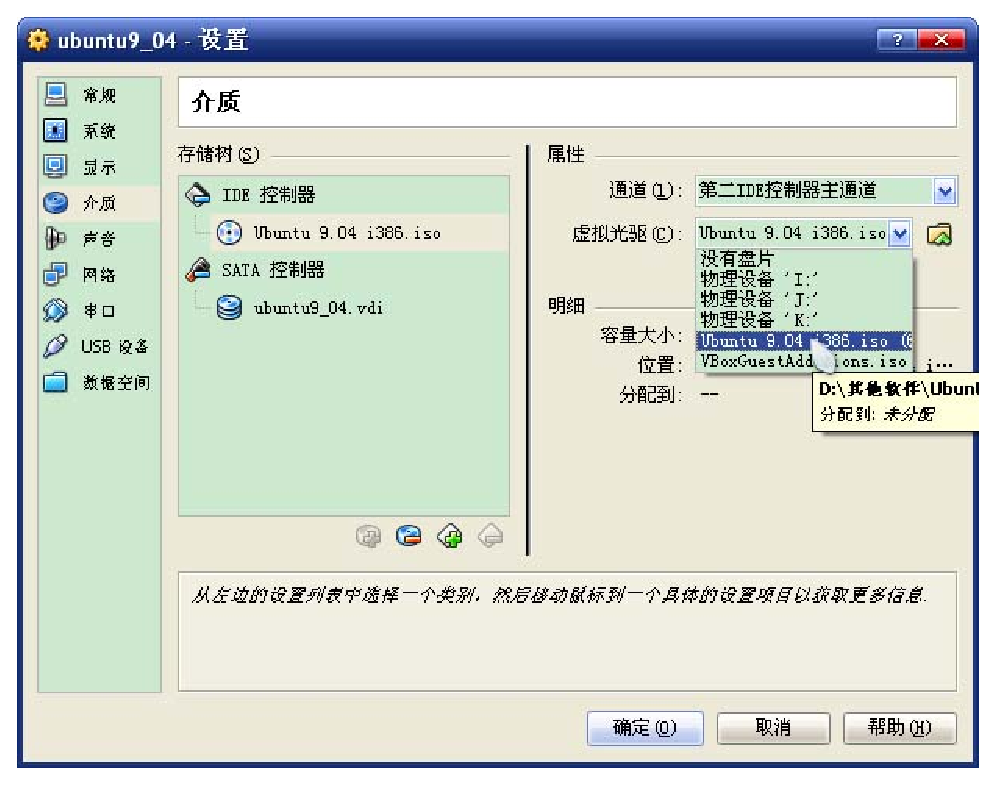
\includegraphics[width=0.8\textwidth,scale=0.8]{pic/f_vb_setting_iso_set.eps}
\caption{设置ISO\label{iso2}}
\end{figure}

之后运行虚拟机,系统就会从ISO进行引导,进而安装Ubuntu系统.过程略.

安装完成后.若宿主机能够访问互联网,则虚拟机也能访问互联网.剩下一个问题就是共享文件夹的设置.在设置之前,需要先安装Virtual Box提供的
增强工具包.在运行虚拟机的界面上选择\fbox{设备-->安装增强功能}.此时在虚拟机的桌面上就会出现一个光盘.打开终端\footnote{Alt+F2调出运行
窗口,输入\fbox{gnome-terminal}回车即可调出终端}.在终端中输入如下命令\footnote{下文中没有特别说明,运行的命令都将是在终端中}:
\begin{verse}
cd /media/cdrom\\sudo ./VBoxLinuxAdditions-x86.run \#若本地PC是amd64位架构,就运行VBoxLinuxAdditions-amd64.run\\输入管理员密码
\end{verse}
等待安装过程结束,关闭虚拟机{\CJKfamily{ht}(注意,这里一定要先关闭虚拟机)}.然后在\fbox{设置}中右侧找到"数据空间",添加一个在宿主机上已经存在的文件夹作为共享目的地.如图\ref{f_sf}所示.
启动虚拟机,终端中输入如下命令:
\begin{verse}
mkdir -p /home/<你的用户名>/Desktop/VBS \#在虚拟机中创建一个文件夹\\sudo mount -t vbox <宿主机中共享文件夹名称> 
/home/<你的用户名>/Desktop/VBS
\end{verse}
经过这番设置后,共享文件夹就设置成功了.但是,重启后设置将会失效,为使启动后系统自动处理共享文件夹,需作如\pageref{cmd0}页所示配置.
\begin{verse}\label{cmd0}
sudo gedit /etc/fstab\\在打开的文件中添加一行" VBoxSharedFolder  /home/<你的用户名>/Desktop/VBS/  vboxsf  defaults 0 0"
\end{verse}
\begin{figure}[!bthp]
\centering
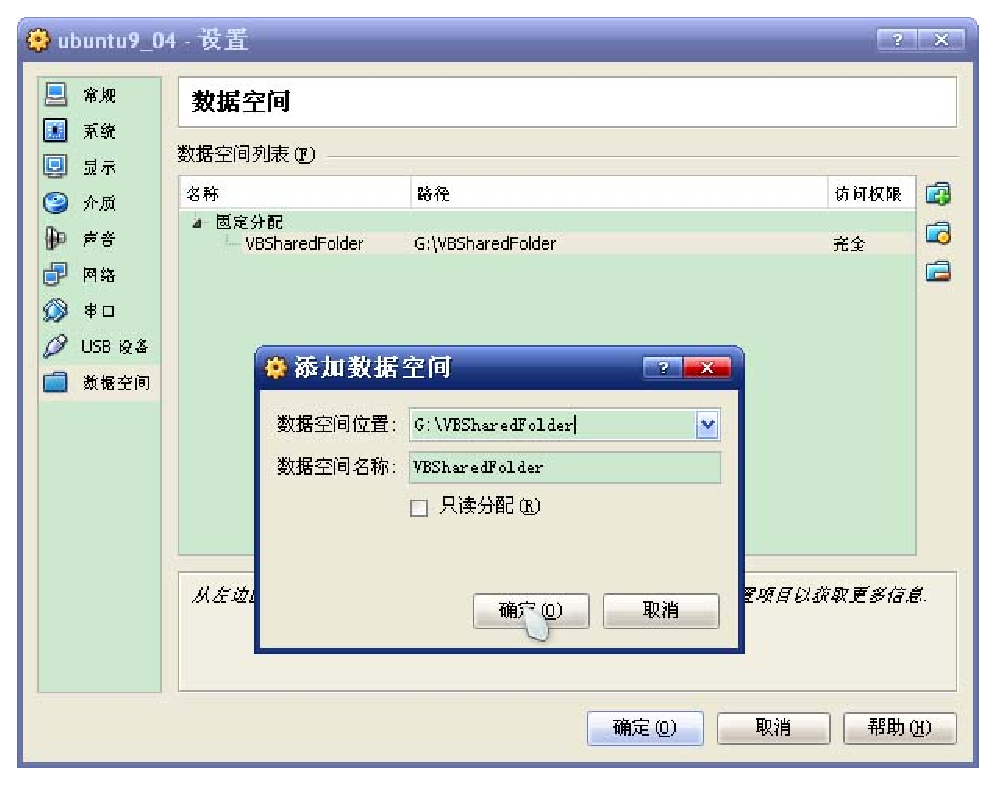
\includegraphics[width=0.8\textwidth,scale=0.8]{pic/f_vb_setting_sf.eps}
\caption{共享空间设置\label{f_sf}}
\end{figure}
%%%2.2.2
\subsubsection{内核开发包安装设置}
在安装内核开发包之前,要先安装一些基本的软件包:
\begin{verse}
sudo apt-get install git-core git-doc automake libtool enca ncurses-dev pax-utils
\end{verse}

将我提供的内核开发包\footnote{nios2-linux\_CF.tgz}拷贝到{\CJKfamily{ht}宿主机}的共享文件夹下,在{\CJKfamily{ht}虚拟机终端}运行如下命令:
\begin{verse}
cd /\\sudo chown <你的用户名,在这里,是bearchen:/> opt/\\mkdir NiosIILinux\\cd /opt/NiosIILinux/\\
tar -zxvf /home/<你的用户名>/Desktop/VBS/<内核开发包名称>
\end{verse}
我们将把内核开发不包安装在/opt目录下,前两个命令的目的是修改opt的所有者,方便之后运行命令.第三个命令则是我的内核开发包历史遗留问题.
地四个命令将内核解压缩到/opt/NiosIILinux/目录下.

{\CJKfamily{ht}注意,接下来的操作比起从官方网站下载的开发包要少一道步骤,就是将源码从git仓库中导出.因为我提供的源码包已经导出相关源码.}
接着安装内核开发所需的工具,包括gcc编译器等(其实就是将工具程序所在文件夹注册到系统环境变量中):
\begin{verse}
gedit ~/.bashrc\\在打开的文件中最后添加一行"export PATH=\$PATH:/opt/NiosIILinux/nios2-linux/toolchain-mmu/x86-linux2/bin"保存修改\\
source ~/.bashrc \#更新环境变量
\end{verse}
通过以上操作,内核开发的软件环境已经搭建完毕.为了测试当前是否搭建成功.可做如下操作:
\begin{enumerate}
\item 运行以下命令:
\begin{verse}
cd /opt/NiosIILinux/nios2-linux/uClinux-dist/\\make clean\\make menuconfig
\end{verse}
在打开的界面中\footnote{这是内核的配置菜单,在这个菜单中,Enter表示进入下一层,ESC两次表示退回上一层或者退出,SPACE表示修改选项状态}
选择"Kernel/Library/Defaults Selection--->"进入.选中"Default all settings(lose changes)".退出保存.对遇到的所有提问选择'N'.
\item 再次运行\fbox{make menuconfig}.进入"Kernel/Library/Defaults Selection--->".选中"Customize Kernel Settings".退出保存.
\item 在新弹出的配置窗口,进入"Device driver--->Network device support--->Ethernet(10 or 100mbit)--->"将"Altera Triple Speed Ethernet 
MAC Support(SLS)"选项取消.退出保存.
\item 运行以下命令\footnote{rc是linux内核启动后会自动执行的脚本文件,
可以通过他人为设置开机后自动运行的命令序列.这里设置为空,避免之后编译出的内核运行时出现不必要的现象.}:
\begin{verse}cd /opt/NiosIILinux/nios2-linux/uClinux-dist/vendors/Altera/common/\\echo > rc\end{verse}
\item 运行\fbox{make}.若接下来的过程没有错误.恭喜你.整个环境已经配置成功.
\end{enumerate}
%%%2.3
\subsection{体验NIOS II Linux}
如果你手头上正好有一块DE2-70开发板,则可以通过以下方式体验一下linux在nios处理器上运行的感觉.
\begin{enumerate}
\item 找到本文附带的文件夹中的两个文件"Starter\_Hardware.sof"和"Starter\_Kernel.gz".将他们拷贝到同一个文件夹下.
\item 运行nios shell.如图\ref{ns}所示.
\item 将DE2-70的电源和usb-blaster连接好.上电.
\item 在nios shell下进入刚才保存两个文件的目录.{\CJKfamily{ht}运行命令}\footnote{注意,这里是在宿主机的nios shell下输入命令}:
\begin{verse}
nios2-config-sof Starter\_Hardware.sof\ {}\ {}\&\&\ {}\ {}nios2-download -g Starter\_Kernel.gz\ {}\ {}\&\&\ {}\ {}nios2-terminal
\end{verse}
在nios shell上打印一堆信息后将看到类似终端的命令提示符.
若一切正常,此时的nios shell将作为开发板上运行的linux内核的终端与用户交互,你可以尝试输入命令获得响应.
\end{enumerate}
\begin{figure}[!htbp]
\centering
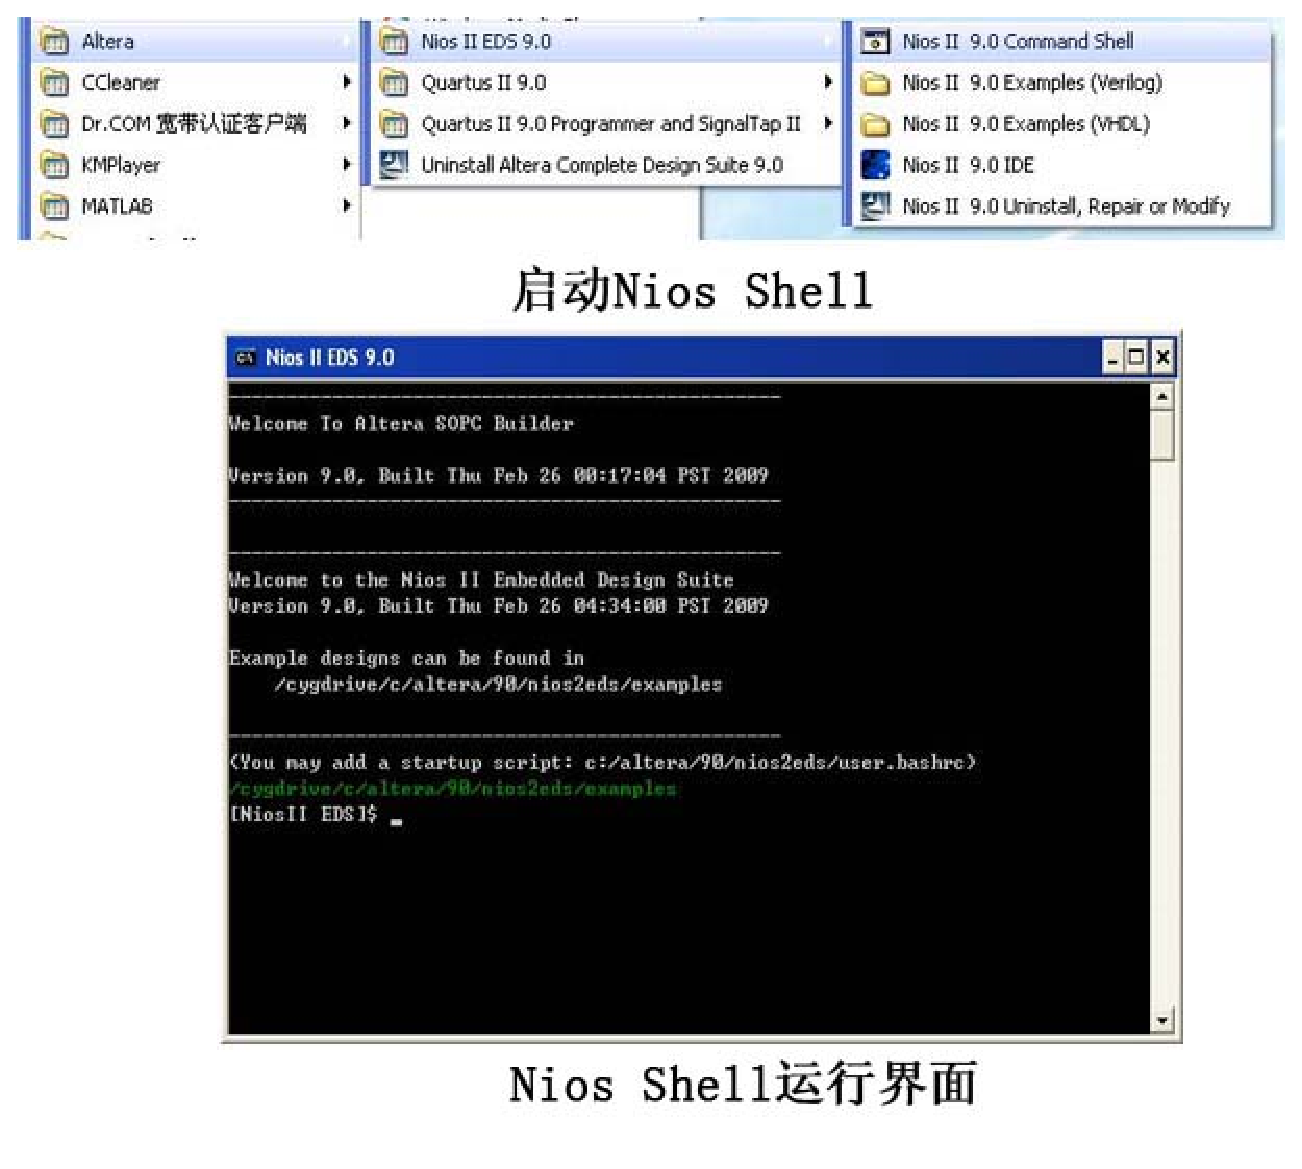
\includegraphics[width=0.75\textwidth,scale=0.75]{pic/f_shell_and_icon.eps}
\caption{Nios Shell图标和运行界面\label{ns}}
\end{figure}
%%%%%%%%%%%%%%%%%%%%走一遍流程%%%%%%%%%%%%%%%
\newpage{}
\section{第一个工程}
\end{document}
